\documentclass{article}
\usepackage{listings}
\usepackage{xcolor}
\usepackage[margin=1in]{geometry}
\usepackage{amsmath,amsthm,amssymb}
\usepackage{graphicx}
\usepackage{epstopdf}
\DeclareGraphicsExtensions{.eps,.ps,.jpg,.bmp}
\lstset{
  numbers=left,
    framexleftmargin=10mm,
    frame=none,
    backgroundcolor=\color[RGB]{245,245,244},
  keywordstyle=\bf\color{blue},
  identifierstyle=\bf,
  numberstyle=\color[RGB]{0,192,192},
  commentstyle=\it\color[RGB]{0,96,96},
  stringstyle=\rmfamily\slshape\color[RGB]{128,0,0},
  showstringspaces=false
    }

\newcommand{\N}{\mathbb{N}}
\newcommand{\R}{\mathbb{R}}
\newcommand{\Z}{\mathbb{Z}}
\newcommand{\Q}{\mathbb{Q}}

\newenvironment{theorem}[2][Theorem]{\begin{trivlist}
\item[\hskip \labelsep {\bfseries #1}\hskip \labelsep {\bfseries #2.}]}{\end{trivlist}}
\newenvironment{lemma}[2][Lemma]{\begin{trivlist}
\item[\hskip \labelsep {\bfseries #1}\hskip \labelsep {\bfseries #2.}]}{\end{trivlist}}
\newenvironment{exercise}[2][Exercise]{\begin{trivlist}
\item[\hskip \labelsep {\bfseries #1}\hskip \labelsep {\bfseries #2.}]}{\end{trivlist}}
\newenvironment{problem}[2][Problem]{\begin{trivlist}
\item[\hskip \labelsep {\bfseries #1}\hskip \labelsep {\bfseries #2.}]}{\end{trivlist}}
\newenvironment{question}[2][Question]{\begin{trivlist}
\item[\hskip \labelsep {\bfseries #1}\hskip \labelsep {\bfseries #2.}]}{\end{trivlist}}
\newenvironment{corollary}[2][Corollary]{\begin{trivlist}
\item[\hskip \labelsep {\bfseries #1}\hskip \labelsep {\bfseries #2.}]}{\end{trivlist}}

\begin{document}

\title{Homework 4}
\author{Chuan Lu\\
13300180056}

\maketitle

\begin{problem}{1}
\text{ }\\
Simulate the random variable X and Y, and estimate E(X) and E(XY).
\end{problem}

\begin{proof}
\section{Answer}
1. Randomly choose $x_{0}$ and $y_{0}$, which obey U(0, B);\\
2. For i in 1:n, \\
2.1 Sample $x_{i+1}$ from $f(x|y = y_{i}) = C(y_{i})e^{-y_{i}x}$; \\
2.2 Sample $y_{i+1}$ from $f(y|x = x_{i+1}) = C(x_{i+1})e^{-x_{i+1}y}$; \\
3. Choose the last $\frac{n}{2}$ samples as a simulation of X and Y; \\
4. $E(X) = \frac{2}{n}\Sigma x_{i}$, for x in the samples mentioned above;
$\quad$ $E(XY) = \frac{4}{n^2}\Sigma_{i}\Sigma_{j} x_{i}y_{j}$, for x and y in the samples in step 3;
\end{proof}


\begin{problem}{2}
\text{ }\\
Estimate (1)$E(X_1+2X_2+3X_3|X_1+2X_2+3X_3>15)$, (2)$E(X_1+2X_2+3X_3|X_1+2X_2+3X_3<1)$ with simulation methods.
\end{problem}
\begin{proof}
\section{Answer}
\subsection{subproblem1}

\end{proof}


\begin{problem}{3}
\text{ } \\
Estimate X, Y, Z and E(XYZ) with the distribution given.
\end{problem}
\begin{proof}
\section{Answer}
\subsection{subproblem1}
1. We have $f(x|y,z) = \frac{f(x,y,z)}{\int_{0}^{\infty} f(x,y,z)dx} = (ay+bz+1)e^{-(x+axy+bxz)}$. \\        
Equally, $f(y|x,z) = (ax+cz+1)e^{-(y+axy+cyz)}$, $f(z|x,y) = (bx+cy+1)e^{-(z+bxz+cyz)}$. \\
2. Randomly select the initial data $x_{0}, y_{0}, z_{0}$, which are all larger than 0. \\
3. For i in 0:n, \\
3.1 Sample $x_{i+1}$ from $f(x|y_{i}, z_{i}) = (ay_{i}+bz_{i}+1)e^{-(1+ay_{i}+bz_{i})x}$;\\
3.2 Sample $y_{i+1}$ from $f(y|x_{i+1}, z_{i}) = (ax_{i+1}+cz_{i}+1)e^{-(1+ax_{i+1}+cz_{i})y}$; \\
3.3 Sample $z_{i+1}$ from $f(z|x_{i+1}, y_{i+1}) = (bx_{i+1}+cy_{i+1}+1)e^{-(1+bx_{i+1}+cy_{i+1})z}$;\\
4. Choose the last half as an estimation of X, Y and Z.
\subsection{subproblem2}
1. Sample X, Y, Z with the process above, in which a, b, c replaced by 1; \\
2. Estimate $E(XYZ) = \frac{8}{n^3}\sum\sum\sum xyz$, in which x, y, z are the samples chosen.
\subsection{the code of subproblem2 is as follows.}
\begin{lstlisting}[language = {R}]
######### Gibbs Sampling for problem 3 ###########
sample3 = function(param1, param2) {
  lambda = 1/(param1 + param2 + 1);
  ##### Using inverse transform algorithm to generate the distribution:
  ##### f(x|lambda) = lambda*exp(-lambda*x);
  u = runif(1);
  x = -lambda*log(lambda*u);
  return(x);
}

gibbs_sampling3 = function(n, init_param) {
  ##### Initialize parameters;
  x = rep(0, n);
  y = rep(0, n);
  z = rep(0, n);
  x[1] = init_param[1];
  y[1] = init_param[2];
  z[1] = init_param[3];
  
  ##### Iterative Sampling;
  for(i in 2:n) {
    x[i] = sample3(y[i-1], z[i-1]);
    y[i] = sample3(x[i], z[i-1]);
    z[i] = sample3(x[i], y[i]);
  }
  rlist = list(x, y, z);
  return(rlist);
}

estimate3 = function(n) {
  res = gibbs_sampling3(2*n, c(1, 1, 1));
  X = res[[1]];
  Y = res[[2]];
  Z = res[[3]];
  X_sample = X[(n+1):(2*n)];
  Y_sample = Y[(n+1):(2*n)];
  Z_sample = Z[(n+1):(2*n)];

  sum = sum(X_sample)*sum(Y_sample)*sum(Z_sample);
  return(sum/(n^3));
}

estimate3(100000)
\end{lstlisting}
\subsection{the result of subproblem2 is as follows}
\begin{lstlisting}[language = {R}]
> estimate3(100000)
[1] 0.4532435
\end{lstlisting}
\end{proof}

\begin{problem}{4}
\text{ }\\
Estimate E(X), E(Y) and E(N) with the distribution given.
\end{problem}
\begin{proof}



\end{proof}

\begin{problem}{5}
\text{ } \\
Generate a mixed normal distribution with the means and covariances given.
\end{problem}
\begin{proof}
\section{Answer}
\subsection{the algorithm}
1. Randomly select the initial vector X and Y. \\
2. For each step: \\
2.1 Generate $X_{i+1}$, $Y_{i+1}$ with $X_{i}$, $Y_{i}$ using Gibbs Sampling. \\
2.2 Generate $u~U(0, 1)$, if $u>0.5$, set Z = X; else Z = Y. \\
3. In detail, in order to generate a 2D normal distribution, we can regard the joint distribution as\\
$$f(x_{1}, x_{2}) = \frac{1}{2\pi\sqrt{\det\Sigma}}e^{\frac{1}{2}(a_{11}(x_{1}-\mu_{1})^{2}+(a_{21}+a_{12})(x_{1}-\mu_{1})(x_{2}-\mu_{2})+a_{22}(x_{2}-\mu_{2})^2)},$$ in which $a_{ij}$ are the elements in $\Sigma$, and $\mu_{i}$ are the elements in $\mu$. \\
3.1 $f(x_{2}|x_{1} = \hat{x_{1}}) = N(\mu_{2}+a_{21}a_{11}^{-1}(\hat{x_{1}}-\mu_{1}),\quad a_{22}-a_{21}a_{11}^{-1}a_{12})$, \\
$f(x_{1}|x_{2} = \hat{x_{2}}) = N(\mu_{1}+a_{12}a_{22}^{-1}(\hat{x_{2}}-\mu_{2}),\quad a_{11}-a_{21}a_{22}^{-1}a_{12})$. \\
3.2 Use Gibbs sampling to generate iteratively X and Y.
\subsection{the code is as follows}
\begin{lstlisting}[language = {R}]
##### Gibbs Sampling for Problem 5 ###
sample5 = function(mu, sigma, x) {
  mean = mu[2]+sigma[2,1]*(1/sigma[1,1])*(x-mu[1]);
  sd = sigma[2,2]-sigma[2,1]*(1/sigma[1,1])*sigma[1,2];
  return(rnorm(1, mean, sd));
}

gibbs_sampling5 = function(n, mu, sigma, init_param) {
  x1 = rep(0, n);
  x2 = rep(0, n);
  x1[1] = init_param[1];
  x2[1] = init_param[2];
  
  mu2 = c(mu[2], mu[1]);
  sigma2 = matrix(c(sigma[2,2], sigma[2,1], sigma[1,2], sigma[1,1]), ncol = 2);
  
  for(i in 2:n) {
    x2[i] = sample5(mu, sigma, x1[i-1]);
    x1[i] = sample5(mu2, sigma2, x2[i]);
  }
  rlist = list(x1, x2);
  return(rlist);
}

simulate5 = function(n) {
  mu1 = c(1, 4);
  mu2 = c(-2, -1);
  sigma1 = matrix(c(1, 0.3, 0.3, 2), ncol = 2);
  sigma2 = matrix(c(3, 0.4, 0.4, 1), ncol = 2);
  
  Z = matrix(rep(0, 2*n), nrow = 2);
  ##### Each col in Z is a sample point #####
  
  X = gibbs_sampling5(2*n, mu1, sigma1, c(1, 1));
  Y = gibbs_sampling5(2*n, mu2, sigma2, c(-3, -3));
  
  x1 = X[[1]];
  x2 = X[[2]];
  y1 = Y[[1]];
  y2 = Y[[2]];

  ##### Take the last half of samples as a simulation ###
  for(i in 1:n) {
    u = runif(1);
    if(u > 0.5) {
      Z[1, i] = x1[i + n];
      Z[2, i] = x2[i + n];
    }
    else {
      Z[1, i] = y1[i + n];
      Z[2, i] = y2[i + n];
    }
  }
  return(Z);
}

n = 10000
z = simulate5(n)
plot(z[1, ], z[2, ])
\end{lstlisting}
\subsubsection{The result is shown as follows}
\begin{figure}[htbp]
\centering
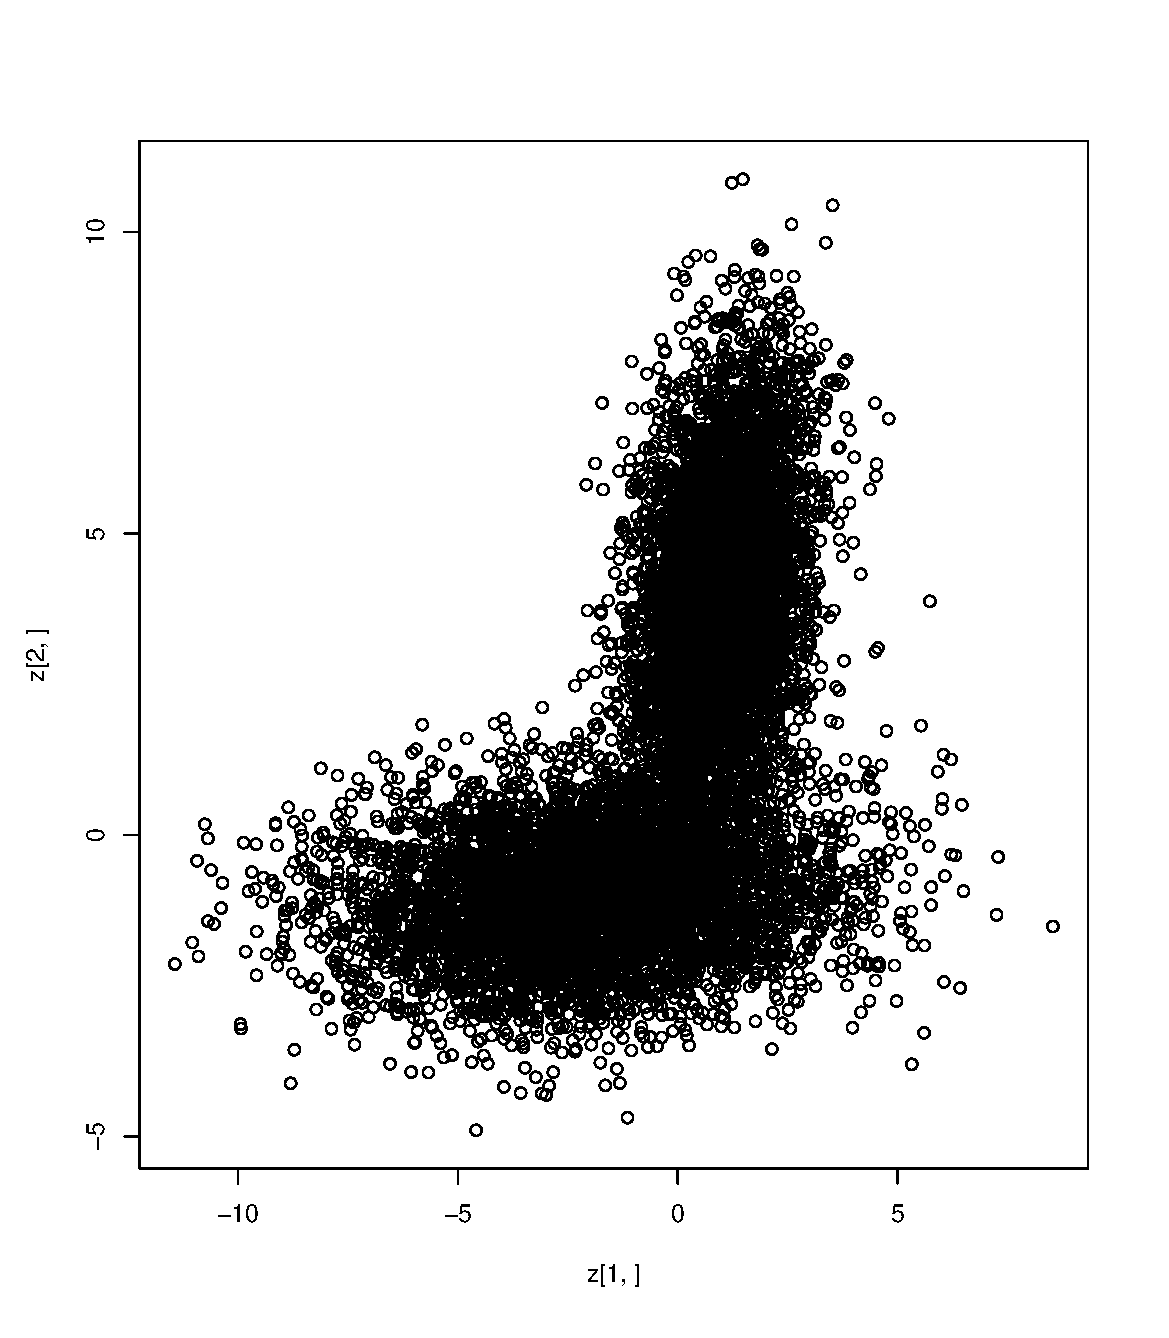
\includegraphics[width = 15cm]{Rplot.eps}
\caption{The simulation of the mixed distribution}
\label{mix}
\end{figure}
\end{proof}
\end{document}
